%*----------- SLIDE -------------------------------------------------------------
\begin{frame}[t]{O problema do transporte no Brasil}
    \vspace{0.5cm}
    \begin{columns}
        \column{.01\textwidth}
        \column{.7\textwidth}
            \begin{itemize}
                \item Roubos de carga crescem no Brasil e prejuízo em 2021 supera R\$ 1,27 bilhão \cite{Roubosdecarga:online}
                \item Pesquisa CNT de Rodovias indica que 59\% da extensão avaliada apresenta problemas; pavimento, sinalização e geometria estão piores \cite{Pioraest:online}
                \item Superlotação de trasporte publico \cite{Superlot45:online}
            \end{itemize}
        \column{.29\textwidth}
            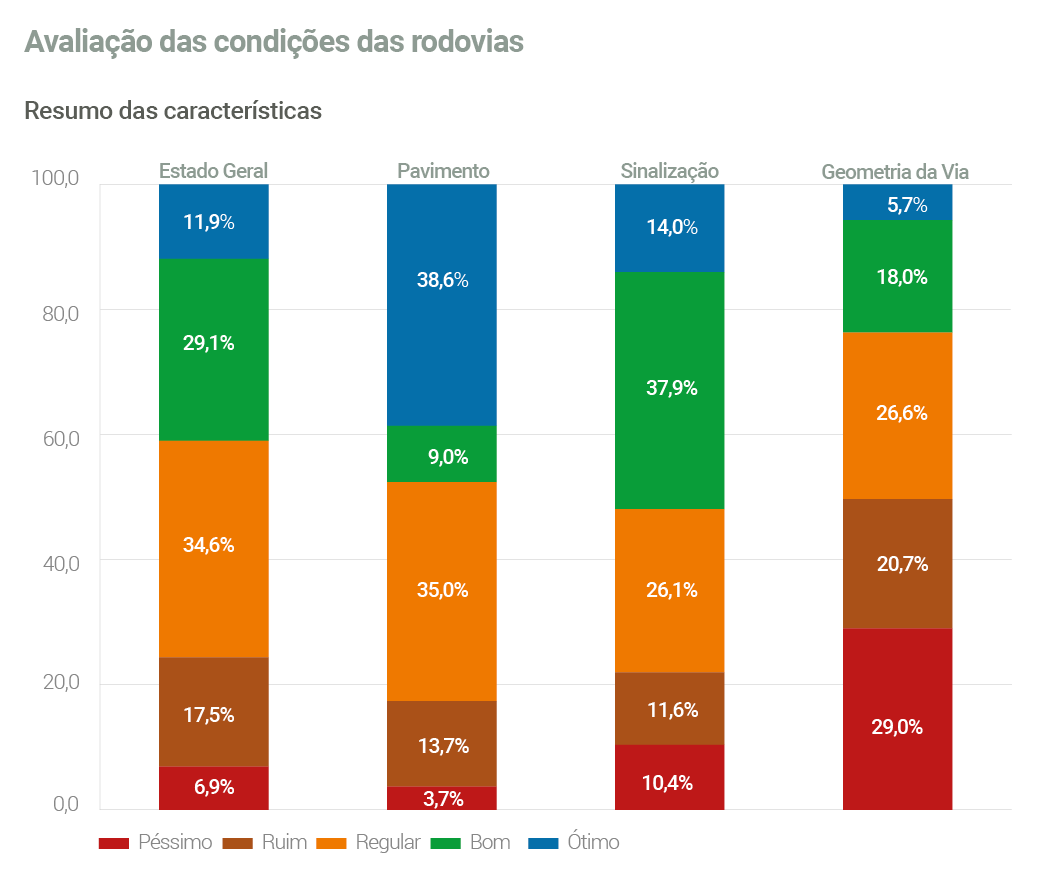
\includegraphics[width=1\textwidth,clip]{transp1.png}
    \end{columns}
    \vspace{1cm}
\end{frame}

%*----------- SLIDE -------------------------------------------------------------
\begin{frame}[t]{O problema do transporte em Salvador}
    \vspace{0.5cm}
    \begin{columns}
        \column{.01\textwidth}
        \column{.7\textwidth}
            \begin{itemize}
                \item Dados levantados junto à Secretaria de Segurança Pública (SSP-BA) apontam que foram registrados em Salvador 1.381 assaltos a ônibus, entre janeiro e outubro deste ano. O número representa uma média de quatro assaltos por dia na capital baiana. \cite{assaltossa:online}
                \item Superlotação do transporte público \cite{Passagei20:online}
                \item Alto custos da passagem
            \end{itemize}
        \column{.29\textwidth}
            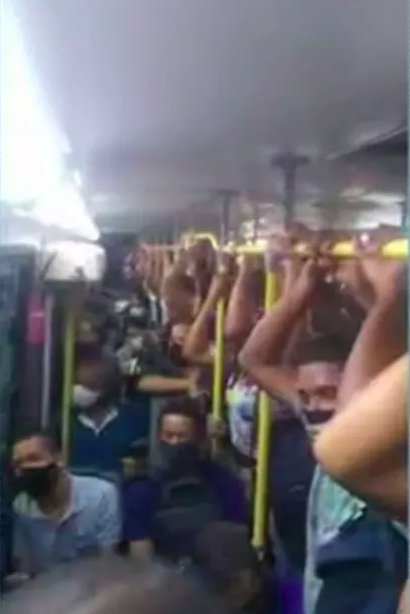
\includegraphics[width=1\textwidth,clip]{buslotado.png}
    \end{columns}
    \vspace{1cm}
\end{frame}
